
The information about all the subjects was collected using a Google form. To maintain participants anonymity, not personal information that could be used to trace them back was collected. The procedure used with each subject is described here below.

\begin{enumerate}
	
	\item The subject was asked to fill out the following information:
	
	\begin{itemize}
		\item Sex
		\item Career
		\item Age
		\item Country of origin.
	\end{itemize}
	
	\item The robot was shown to the participant and the experiment procedure is explained.

	\item An example of the questionnaire was presented and a sample movement of the robot shown.

	\item The subject is exposed to a specific movement sequence according to the following steps:

	\begin{enumerate}

		\item The subject is exposed to the movement generated by a configuration of values.

		\item The subject could use as much time as needed to select values for intensity of the different terms in the questionnaire.

		\item After the subject had completed his/her selection about the current movement, the sequence is repeated for the rest of movements.

	\end{enumerate}
\end{enumerate}

The order of the options enlisted in the questionnaire changed for each question to prevent any kind of bias. Figure~\ref{fig:questionnaire_example} shows an example of the questionnaire used. The experiment was performed at Politecnico di Milano, involving subjects with different backgrounds. %campus Leonardo during the months of June and July of 2015.  
A total of 49 volunteers were involved: 12 females and 37 males. The average age of the subjects was 25.28, with standard deviation of 2.8, with a minimum age of 20 and maximum of 32. The subjects' country of origin and their backgrounds are shown in the Table~\ref{table:country} and Table~\ref{table:career}, respectively. 

\begin{figure}
	\centering
	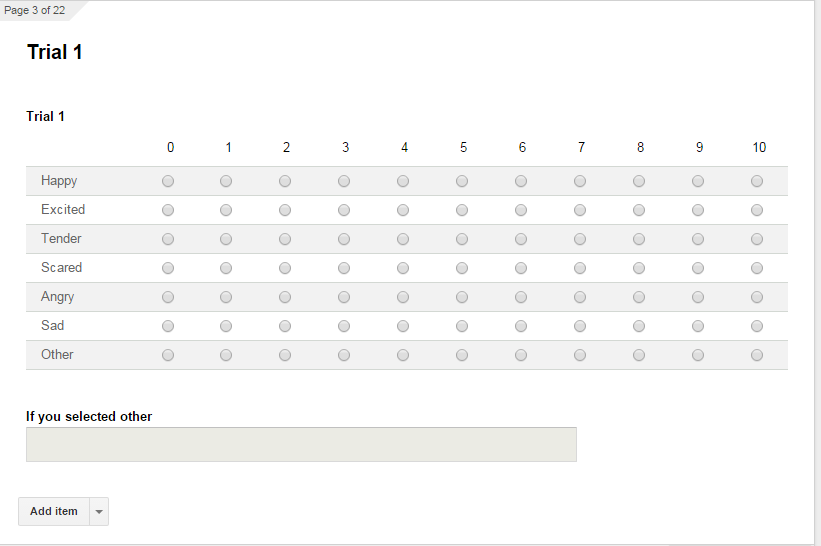
\includegraphics[width=0.48\textwidth]{./Images/example_survey.png} 
	\caption{Example of the questionnaire used in the experiment.}
	\label{fig:questionnaire_example}
\end{figure}

%%%%%%%%%%%%%%%%%%%%% 
\begin{table}[h]
\centering
\caption{Subjects' Country of origin.}
\label{table:country}
\begin{tabular}{|c|c|}
\hline
\textbf{Country} & \textbf{Counting} \\
\hline
Albania & 1 \\
\hline
Bosnia & 1 \\
\hline
Brazil & 2 \\
\hline
Colombia & 4 \\
\hline
Germany & 1 \\
\hline
Greece & 1 \\
\hline
Iran & 5 \\
\hline
Italy & 33 \\
\hline
Moldova & 1 \\
\hline 
\multicolumn{2}{c}{}
\end{tabular} 
\end{table}
%%%%%%%%%%%%%%%%

\begin{table}[h]
\centering
\caption{Subjects' Background.}
\label{table:career}
\begin{tabular}{|c|c|}
\hline
\textbf{Career} & \textbf{Counting}\\
\hline
Aeronautical Engineering & 1 \\
\hline
Architecture & 1 \\
\hline
Social assistance & 1 \\
\hline
Automation & 1 \\
\hline
Bio-medical Engineering & 5 \\
\hline
Computer Science & 33 \\
\hline
Electronic Engineering & 2 \\
\hline
Mechanical Engineering & 2 \\
\hline
Nursery & 1 \\
\hline
Pedagogical Science & 1 \\
\hline
Tourism & 1 \\
\hline
\multicolumn{2}{c}{}
\end{tabular} 
\end{table}